\subsection{Equipment} %
\noindent When participating in RoboSub, there is some equipment needed to be present on the AUV in order to fulfill all the goals of the competition. Naiad will therefore be equipped with two markers, two torpedoes and a pair of grippers. Additionally, there will also be two speed loggers equipped, one mounted on the tool plate and the other on the lid. This section will discuss the design and implementation of each of these tools and how they can be further developed.   

\subsubsection{Speed logger} %Lennie
\label{SL_mec}
Since Naiad has trouble determining its position in water when there is nothing to navigate after, a speed logger was built. The speed is calculated from a sensor that measures how fast the turbine is rotating in the pipe. The speed logger has seven main parts and three screws. The base plate is formed so that water will easily flow into the pipe where the turbine is mounted. The pipe is built out of a plexi tube and this is the only part except for the screws that is not created with a 3D-printer. The pipe exists so that the flow of water is only measured in one direction, otherwise the water flowing from the sides might disrupt the speed values in a certain direction. The turbine is built so that it will be as light as possible for it to be able to spin easily and another goal is that no water flow should get passed it without making the turbine spin. The turbine is held in place by the use of an axle connected to a wheel bearing that is mounted in a centerpiece. The centerpiece has three legs so it will be stable and at the same time not disrupt to much of the water flow. It is held in place in the pipe by the use of 3 screws. Finally the centerpiece has a cap on the other side from the turbine, this is to make the water flow better and to protect the wheel bearing.  The assembly of the speed logger can be seen in fig. \ref{SpeedloggerImg}.

\begin{figure}[!ht]
	\begin{center}
		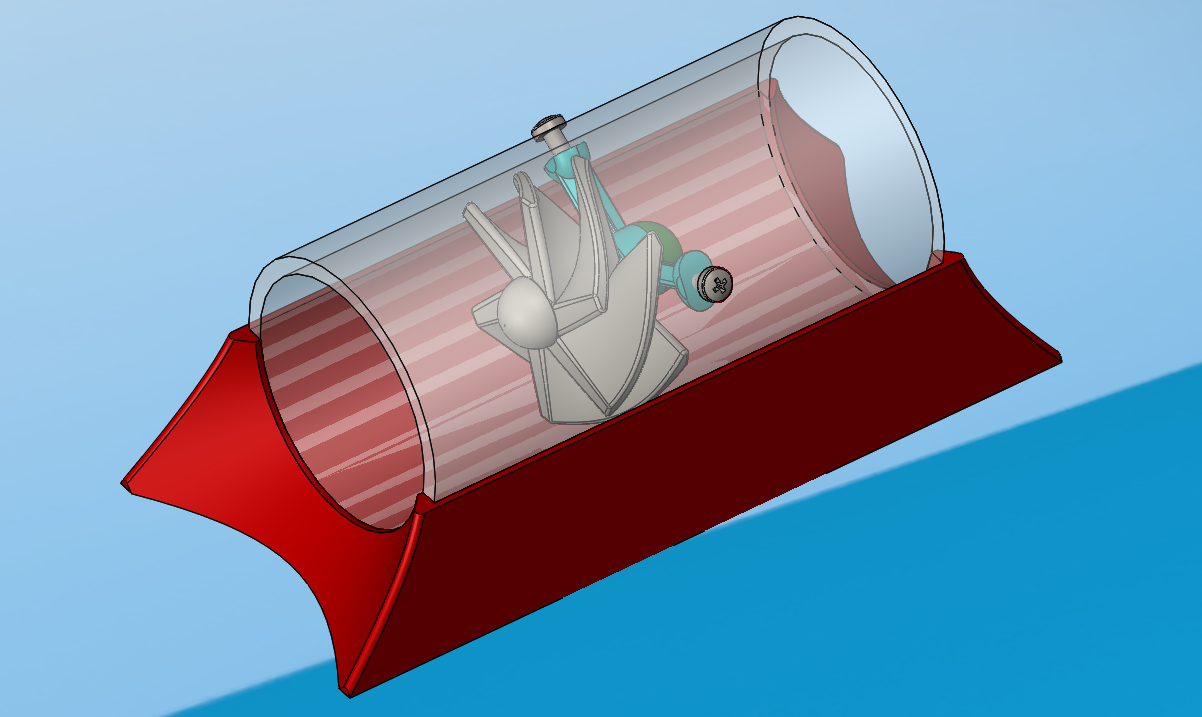
\includegraphics[width=80mm]{./Images/Mechanics/SpeedloggerImg.png}
		\caption{Assembly of the speed logger}
		\label{SpeedloggerImg}
	\end{center}
\end{figure}

\subsubsection{Markers}
	\noindent Naiad should be equipped with two droppable markers. This requirement is for the RoboSub competition. The previous design of the marker assembly consists of two PMMA pipes, one short and one longer, each connected to a top and a bottom plate. The short tube is connected to the top plate on which there are screw holes for attachment to the tool plate. The bottom plate acts as a stabilizing bottom and holder for the other pipe. The design can be seen in fig. \ref{helluuu}. 
	
	\begin{figure}[!ht]
	\begin{center}
		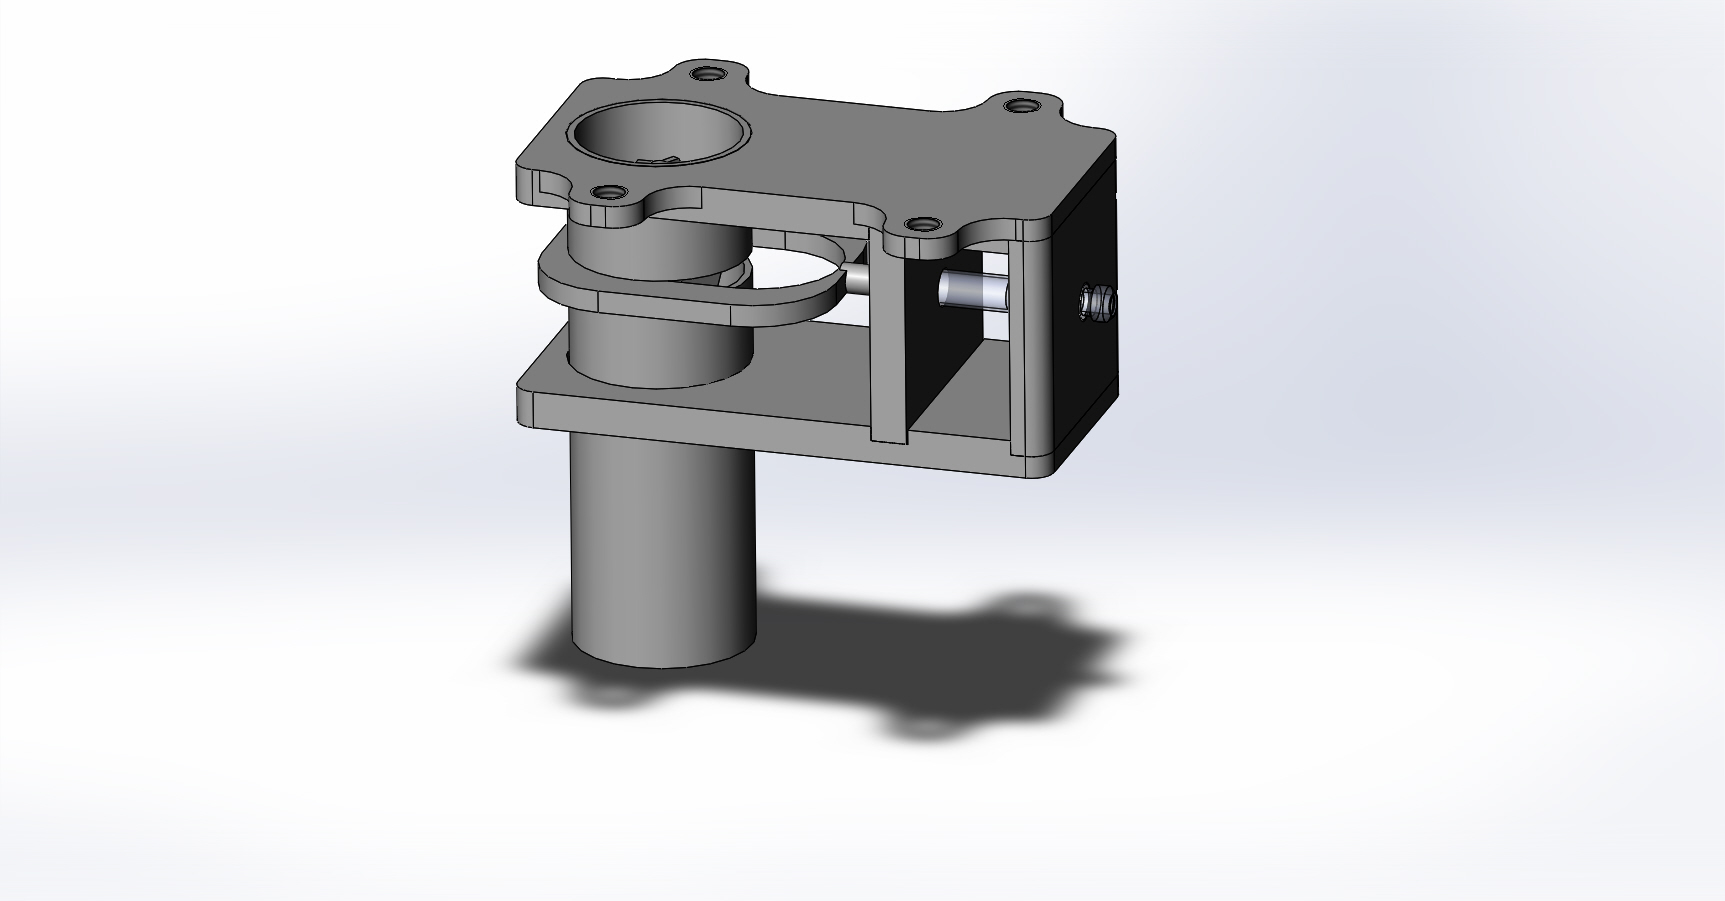
\includegraphics[width=80mm]{./Images/Mechanics/Markerassem3.jpg}
		\caption{The previous version of the marker assembly.}
		\label{helluuu}
	\end{center}
\end{figure}

According to the old design they are to be operated by a pneumatic system. However, it was decided that using pneumatics for the markers would be over complicated for the sole purpose of moving a releaser a few millimeters back and forth. Thus, it was considered if it was possible to replace the pneumatics by using solenoids to release the markers instead. It was considered a good idea and the system was therefore replaced. This meant that the design of the marker holder needed to be adjusted as the existing design of the marker holder would be too large and therefore not fit in the tool plate. A new system with solenoids has not yet been tested as it is still in the planning phase.  

With this new system for dropping the markers, the markers also had to be modified to fit in. A loop was added to the end of the marker so that it could be hanged onto the solenoid pin. Additionally, the shape of the marker had to be changed as the previous marker consisted of a sphere with fins and this design made no room for adding the loop to the marker. See fig. \ref{MarkerPics} for the old and the new design respectively.

\begin{figure}[!ht]
	\begin{center}
		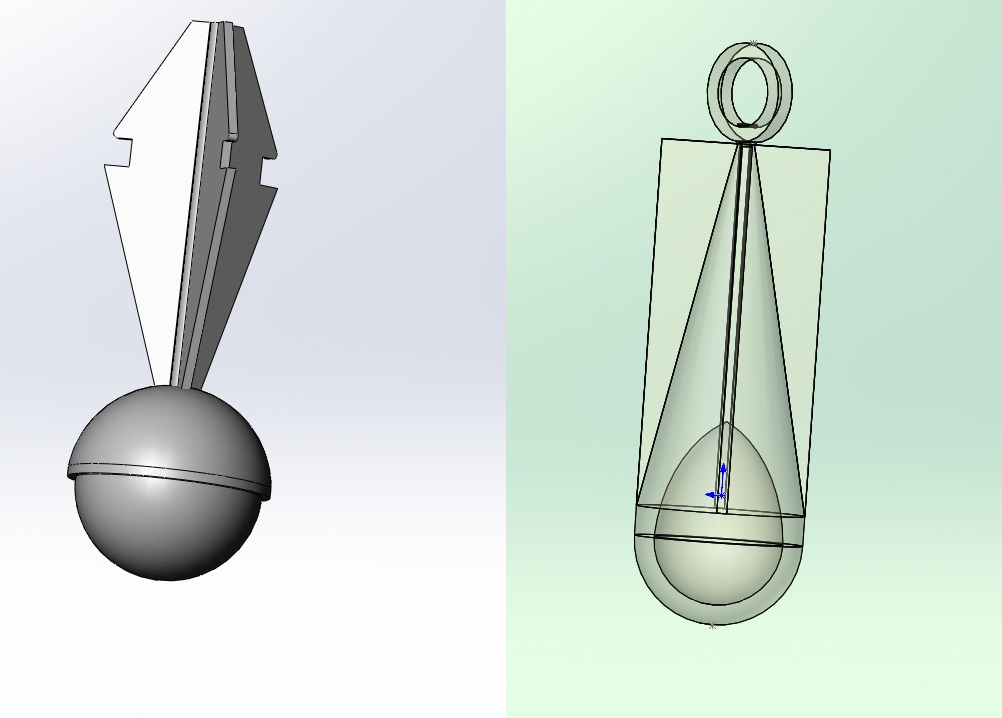
\includegraphics[width=80mm]{./Images/Mechanics/FirstAndSecondMarker.jpg}
		\caption{To the left is the first version of the marker and to the right is the second version of the marker.}
		\label{MarkerPics}
	\end{center}
\end{figure}

The markers now work in such a way that they are activated by a solenoid retracting a pin which the marker hangs onto. The marker will then fall down and out of the pipe. The markers should be heavy in the bottom so that they do not float up to the surface or stay still after release. There were a couple of different tests made to see if the marker was heavy enough to sink relatively straight down, with different methods of making it heavy. As this was made late in the project, a solution for making the markers heavy had to include using items that were easily accessible in order to test them in time. The first method was to add some short screws to the bottom of the markers while they were 3D-printed. However, this created air bubbles inside the marker and also the screws did not create a uniform and balanced mass. This lead to that the markers drifted heavily when being dropped into water. Another idea was to make the marker hollow in the bottom and print the marker in two parts, where each part had a hollow part in the shape of half of a sphere. Then, plaster would be added to each part to fill up the holes. They would then be glued together and a layer of glue was added to the whole bottom part of the marker in order to protect the plaster from water. There were two prototypes made of this solution, one marker with fins and another without fins. When tested in water, the marker without fins worked much better. However, it did not move ideally as it still drifted to some degree. To read more about the placement of the markers with their holders, see section \ref{Markerss}. 


\subsubsection{Torpedeos}
\label{torpedosection}
The basic idea of the torpedo launcher is that a small tube is attached to a plexi tube and the torpedo is mounted inside the plexi tube by a small hole behind the torpedo where the small tube comes in. The torpedo is then attached and stable inside the launcher waiting to fire. By a pneumatic system a pressure goes through the small tube to the torpedo which pushes the torpedo away, see the fig. \ref{torplunch}. However, since markers and new gripper will not use the pneumatic system, it is decided to also use solenoid for the torpedoes. The design of a solenoid torpedo have not yet been designed.


	\begin{figure}[!ht]
		\begin{center}
			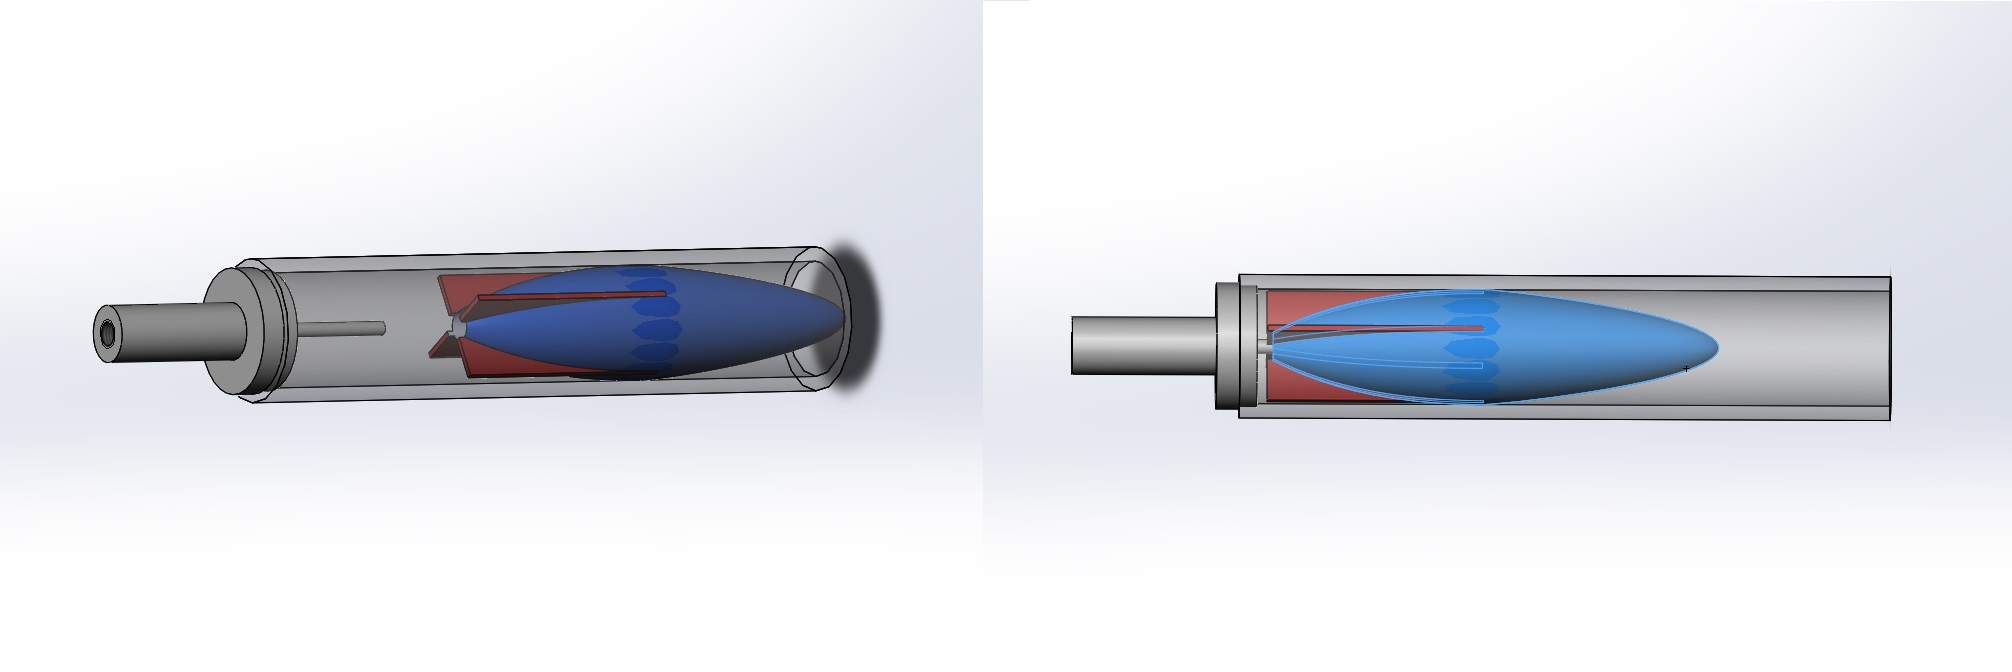
\includegraphics[width=150mm]{./images/mechanics/OverallAssem2.JPG}
			\caption{The torpedo launcher.}
			\label{torplunch}
		\end{center}
	\end{figure}

